%\begin{tikzpicture}[scale=2.2,transform shape]
\begin{tikzpicture}
    \node[anchor=south west,inner sep=0] at (0,0)
        {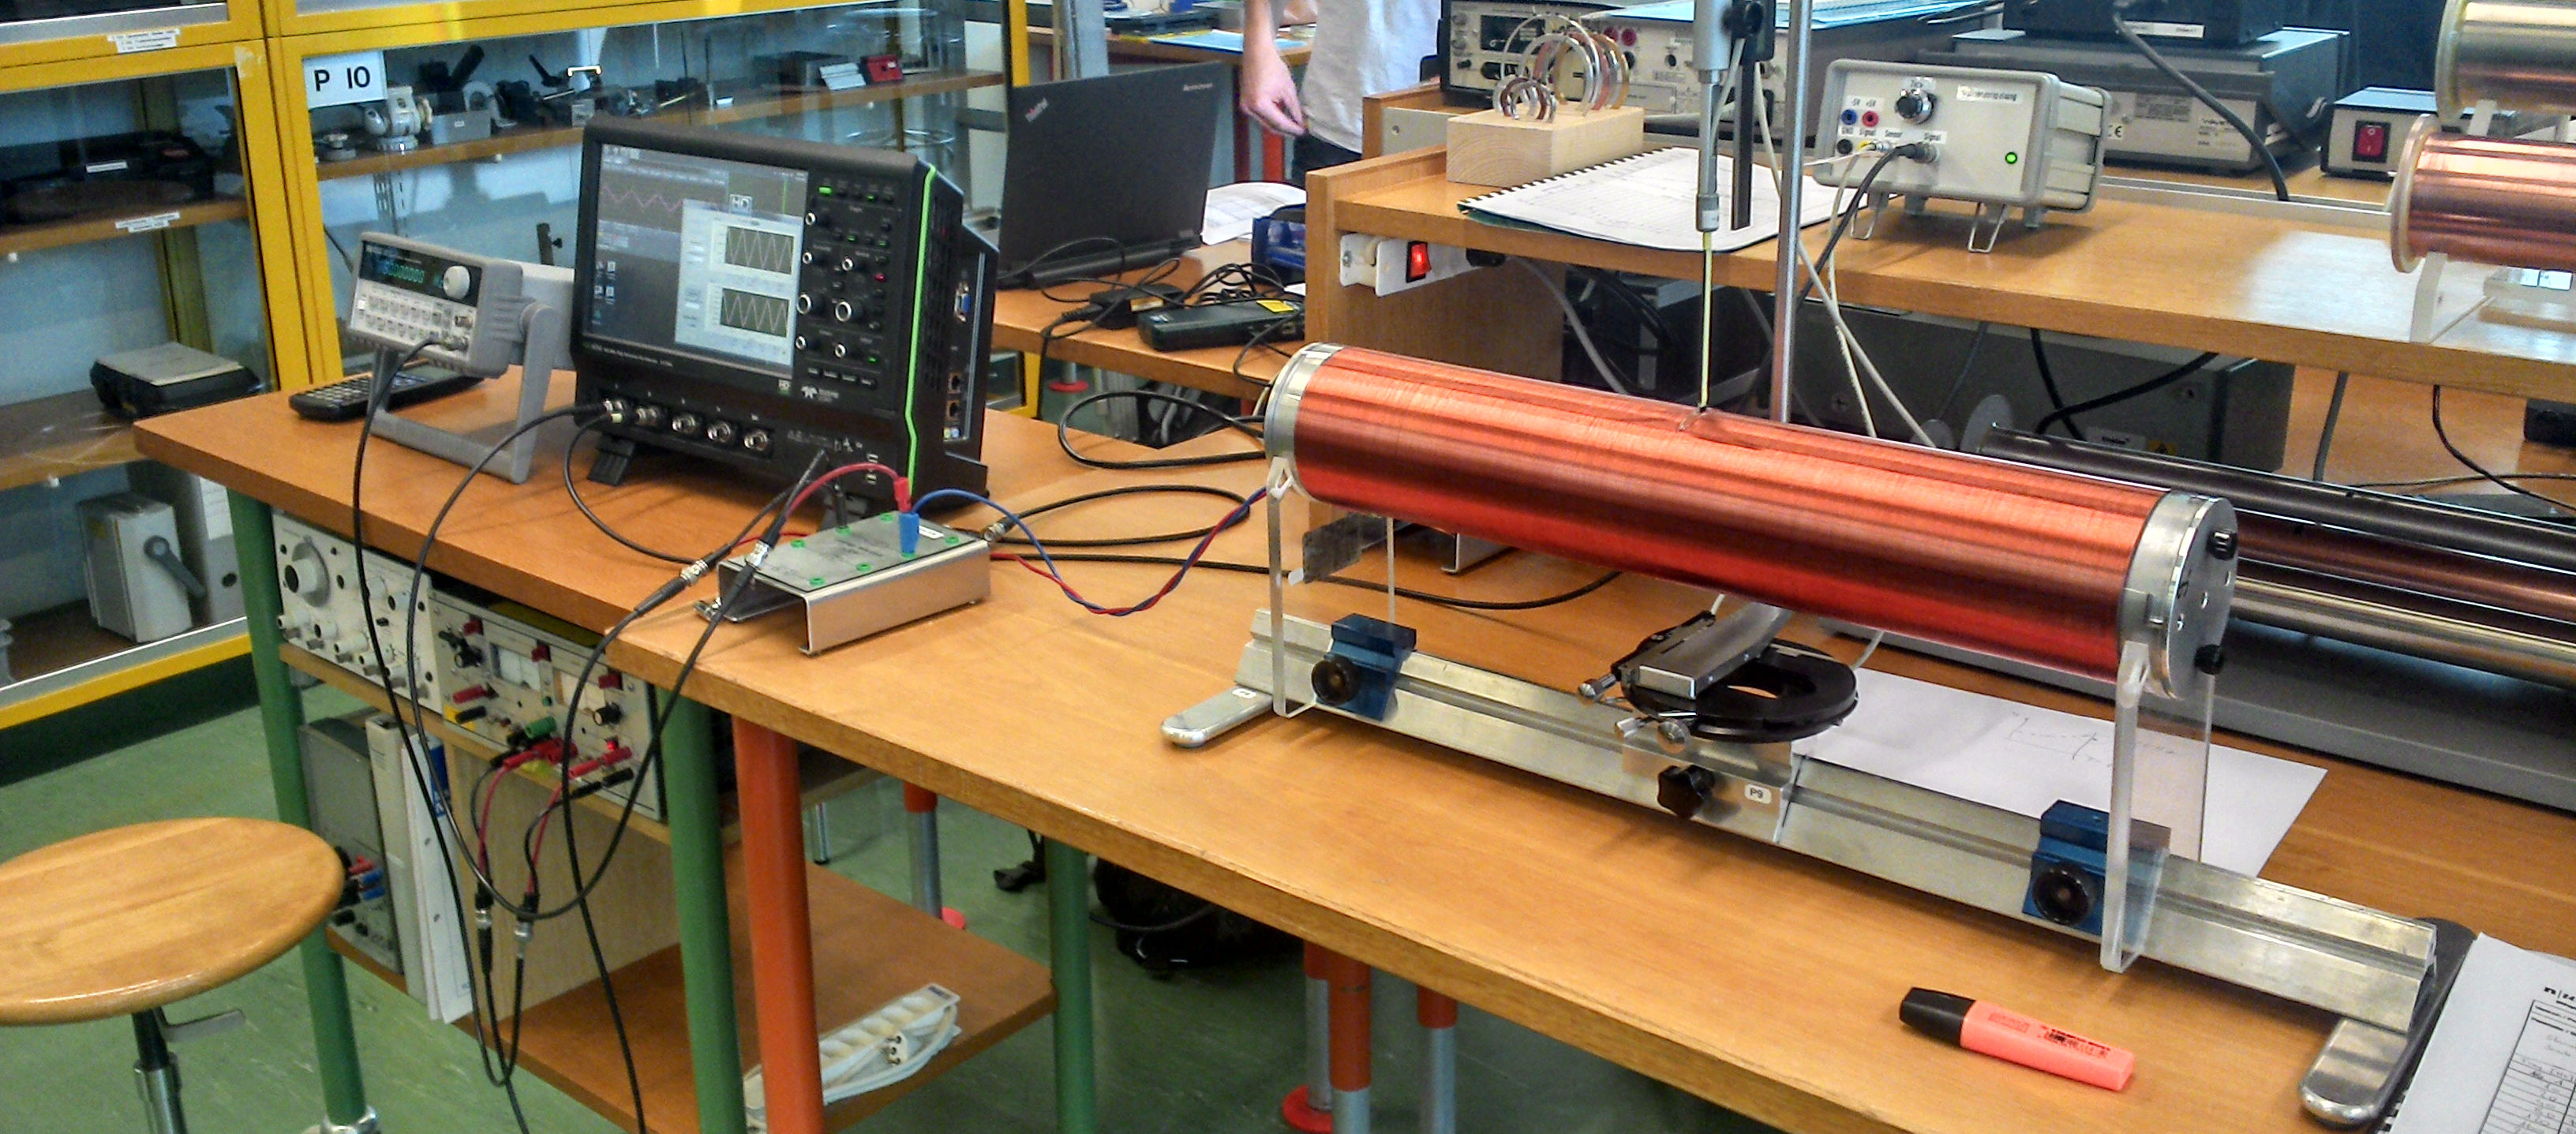
\includegraphics[width=\textwidth]{images/versuchsanordnung-2.jpeg}};

    %\draw[help lines] (0,0) grid (\textwidth,7);

    \fill[black,opacity = 0.6,rounded corners] (1.6,1.7) rectangle (2.2,2.5);
    \draw[white,ultra thick,rounded corners] (1.6,1.7) rectangle (4,3);
    \node at (1.9,2.15) {\huge{\textcolor{white}{2}}};

    \fill[black,opacity = 0.6,rounded corners] (8,4.5) rectangle (9,5.3);
    \draw[green,ultra thick,rounded corners] (8,4.5) rectangle (11.6,5.9);
    \node at (8.5,4.875) {\huge{\textcolor{green}{5,6}}};
\end{tikzpicture}
